\documentclass{sigplanconf}

\usepackage{amsmath}
\usepackage{listings}
\usepackage{graphicx}

\graphicspath{ {figures/} }

% I copied some formatting settings from another template I have used for homework in the past, but I don't like
% how it does comments and will change the formatting.
\lstset{
    language=Java,
    basicstyle=\ttfamily\small,
    aboveskip={1.0\baselineskip},
    belowskip={1.0\baselineskip},
    columns=fixed,
    extendedchars=true,
    breaklines=true,
    tabsize=4,
    prebreak=\raisebox{0ex}[0ex][0ex]{\ensuremath{\hookleftarrow}},
    showtabs=false,
    showspaces=false,
    showstringspaces=false,
    numberstyle=\small,
    stepnumber=1,
    numbersep=10pt,
    captionpos=b,
    escapeinside={\%*}{*)}
}


\begin{document}

\special{papersize=8.5in,11in}
\setlength{\pdfpageheight}{\paperheight}
\setlength{\pdfpagewidth}{\paperwidth}

\title{Preventing Errors in Numerical Computations}
\subtitle{The Unsignedness Checker}

\authorinfo{Christopher A. Mackie}
           {University of Washington}
           {mackic@cs.washington.edu}

\maketitle

% I was mostly aiming to get concepts on paper with this draft. Therefore at this time I am more
% concerned with content than structure. I don't know how much I should focus on the tool itself.
% I think the unique part of this project concerns the construction of a type system which conforms
% to Java's language specifications concerning signedness, that is the assumption that everything is
% signed. I've tried to focus on the type system because of this, but I think I should probably say
% more about the tool. I'm not sure if Approach and Uniqueness should include more content on the
% tool, or if that is best kept for Results and Contributions. I don't know how much background to
% give about unsigned numbers themselves since most people know them, but they are often hidden
% behind several layers of abstraction so maybe a brief blurb like below is necessary to jog
% memories.

\section{Problem and Motivation}

A large class of errors in software can be traced to the mishandling of unsigned integers, those represented at the bit level as pure base two integers. Such numbers are always non-negative and are used to allow for a larger positive range of values to be represented with fewer bits. Because only non-negative numbers can be represented with unsigned integers, the use case for them is relatively rare, and often for low level systems applications, whichare critical pieces of software.\\
\indent
We will use the terms sound and unsound in this paper to discuss operators. When we refer to sound operators, we mean operators whose implementations are agnostic to the signedness of their inputs and outputs, so long as signedness is consistent. Unsound operators, conversely, must have different implementations for each signedness. See Listing 1 for an example of sound and unsound operators.\\

% Sound and unsound may not be the best terms for these concepts, but I thought its a useful concept to talk
% about. A distinction definitely exists between these kinds of operators, which is convenient to put into words
% before discussing type rules.

\begin{lstlisting}[caption=Example depicting subtraction\, a sound operator\, and division\, an unsound operator.]
byte x = 255;
byte y = 254;

byte sub = x - y;
// Unsigned: 1 (Correct)
// Signed: -3 (Correct)

byte div = y / x;
// Unsigned: 2 (Wrong)
// Signed: 2 (Correct)
\end{lstlisting}

\indent
Bugs concerning unsigned integers can easily be divided into three categories. First is those which result from using an unsound operator with operands of the opposite signedness to the implementation of the operator. Another is those which result from mixing signed and unsigned integers while using any operator, sound or unsound. This includes interpreting the result of some operator on unsigned values as signed, or feeding a signed and unsigned integer into an operator. The final category comes from interchanging signed and unsigned integers in routine calls or outputs.\\
\indent
The first line of defense against most bugs is the compiler. When the compiler is unable to catch bugs it falls on the programmer to identify and eliminate them, which is prone to human error. Because Java has unsigned integers, its compiler has no concept of signedness; it is impossible to find any bugs related to using unsigned numbers at compile time using javac. Many programmers attempt to use unsigned numbers in their Java programs despite this, but such efforts are not directly supported by the language and therefore are subject to bugs which arise from human error.\\

\section{Background and Related Work}

% Maybe talk about the checker framework here? I'm not quite sure what to talk about.

\section{Approach and Uniqueness}

Our approach to solving this issue is to use a type system. This allows us to build on Java's current type system and javac's ability to process it in order to perform static analysis on the usage of unsigned integers in Java programs using pluggable type systems. This allows users to catch bugs before they become problems for their end-users. Additionally, this allows us to take a sound approach to catching unsignedness related bugs, that is it allows us to ensure that if a program type-checks it does not contain any bugs concerning unsigned integers. This can be done by always preferring false negatives to false positives.

\begin{figure}
    \centering
    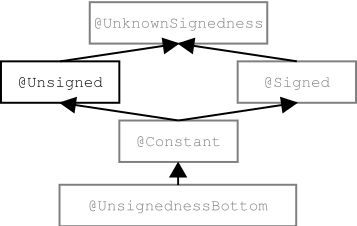
\includegraphics[width=0.4\textwidth]{unsignedness}
    \caption{The type qualifier hierarchy of the Unsignedness annotations.
Qualifiers in gray are used internally by the type system but should never be written by a programmer.}
    \label{fig:my_label}
\end{figure}

The Unsignedness Type System consists of one user defined type, Unsigned, and four internally used types, UnknownSignedness, Signed, Constant, and UnsignednessBottom, and is designed to naturally eliminate the third class of unsigned bugs, the interchange of signed and unsigned integers, by the nature of its hierarchy, shown in Figure~\ref{fig:my_label}.\\
\indent
Types are introduced into a program either by the user, for Unsigned values, or by the the Unsignedness Checker using its type introduction rules. The default type for all symbols is UnknownSignedness, which is also the top type. This type is intended to remain only for types which are transparent to signedness, such as \texttt{String}. If a type is integral, such as \texttt{byte}, \texttt{short}, \texttt{int}, or \texttt{long}, it is defaulted to Signed. If a value is constant at compile time, that is it is a literal or computed from literals, it is Constant. All types are propagated up through operators using Lowest Upper Bound, an approach in which the lowest type in the type hierarchy which is a supertype of all constituent symbols becomes the type of the expression.\\
\indent
The real work of the Unsignedness Type System is done by its type rules, which eliminate the first two classes of bugs associated with unsigned integers. These rules are that no unsound operator may act on Unsigned values, and that Signed and Unsigned values may not be mixed in any operation, sound or unsound. A special exception to the second rule is made for shifts as they behave in a different manner. The second argument to shifts is a modifier to the operator, and as such does not need to match the first argument in signedness. Therefore shifts are tied to their first argument. For example, logical right shifts should operate on Unsigned values, arithmetic right shifts on Signedv values, and left shifts on either.\\
\indent
The Unsignedness Type System is unique in that it must conform to a language specification which assumes that all values and operators are signed. This means that the type system must be more strict than comparable systems in other languages as the assumptions made cannot be altered. To comply with this constraint, we have used a policy of favoring false negatives over false positives to ensure the soundness of the system.


% Also maybe talk about implementation in this section, don't know how much detail on this to use.

\section{Results and Contributions}

% Maybe talk about jake2 here. The case study is not finished so I don't know if its useful to talks about an
% unfinished case study

\bibliographystyle{abbrvnat}

% The bibliography should be embedded for final submission.

\begin{thebibliography}{}
\softraggedright

\bibitem[Smith et~al.(2009)Smith, Jones]{smith02}
P. Q. Smith, and X. Y. Jones. ...reference text...

\end{thebibliography}


\end{document}
